\section{Experiments}\label{sec:exp}



\subsection{Datasets and Baselines}

To show the effectiveness of our method, we use MERL \cite{Matusik2003jul} and RGL (51 isotropic materials) \cite{dupuy2018adaptive} datasets, which are the most commonly used BRDF datasets that include isotropic materials. The MERL dataset \cite{Matusik2003jul} consists of 100 real-world materials, covering a wide range of appearances. Each material includes reflectance measurements from a dense set of directions, parameterized as the spherical angles ($\theta$, $\phi$) of the $H$ and $D$ vectors from the Rusinkiewicz parameterization \cite{rusinkiewicz1998new}. Each color channel has a resolution of 90 × 90 × 180, leading to $1\,458\,000$ reflectance measurements. 



\subsection{Sparse BRDF Reconstruction}\label{sec:brdf_rec}
 For comparison with baselines, we train our hypernetwork model with 80 MERL materials that are randomly selected. We leave the remaining 20 materials for testing. To understand the reconstruction capacity of our model, we first train the model with all available samples ($1\,458\,000$). We observe that reducing the number of samples by around half ($640\,000$) results in a similar performance (Section 7 in supplementary). 

We also train our model with a mixed dataset of 80 MERL materials and 51 isotropic RGL materials. We later test the trained model on the same test dataset (20 MERL materials). We apply a separate log relative mapping to RGL materials by computing the median over the isotropic RGL dataset.
 
 We qualitatively compare our results against the ground truths through renderings of the materials. The renderings are obtained by a Mitsuba renderer with an environment map illumination. Our model can capture the diffuse colors of varying unseen appearances even for the materials with specular components. 



The main advantage of our architecture is that it is flexible in the number of samples fed to the network. That is, we can reconstruct unseen materials with fewer samples than the sample number used during training. Thanks to its built-in nonlinear interpolation that comes from the hyponet, we obtain high quality reconstruction results with fewer samples. 

Considering our architecture, we understand that the gap between reconstruction results with sparse samples relies on the embeddings $z$ (latent vectors). We hence analyse the embeddings for the materials reconstructed with varying number of samples. In Figure \ref{fig:tsne-vis-imputation}, we visualize 
the t-SNE clustering of the test embeddings with different number of samples. It is visible that the embeddings of the same material reconstructed with different sample sizes lie close in the t-SNE space.

\begin{figure}[t]
  \centering
  % \fbox{\rule{0pt}{2in} \rule{0.9\linewidth}{0pt}}
   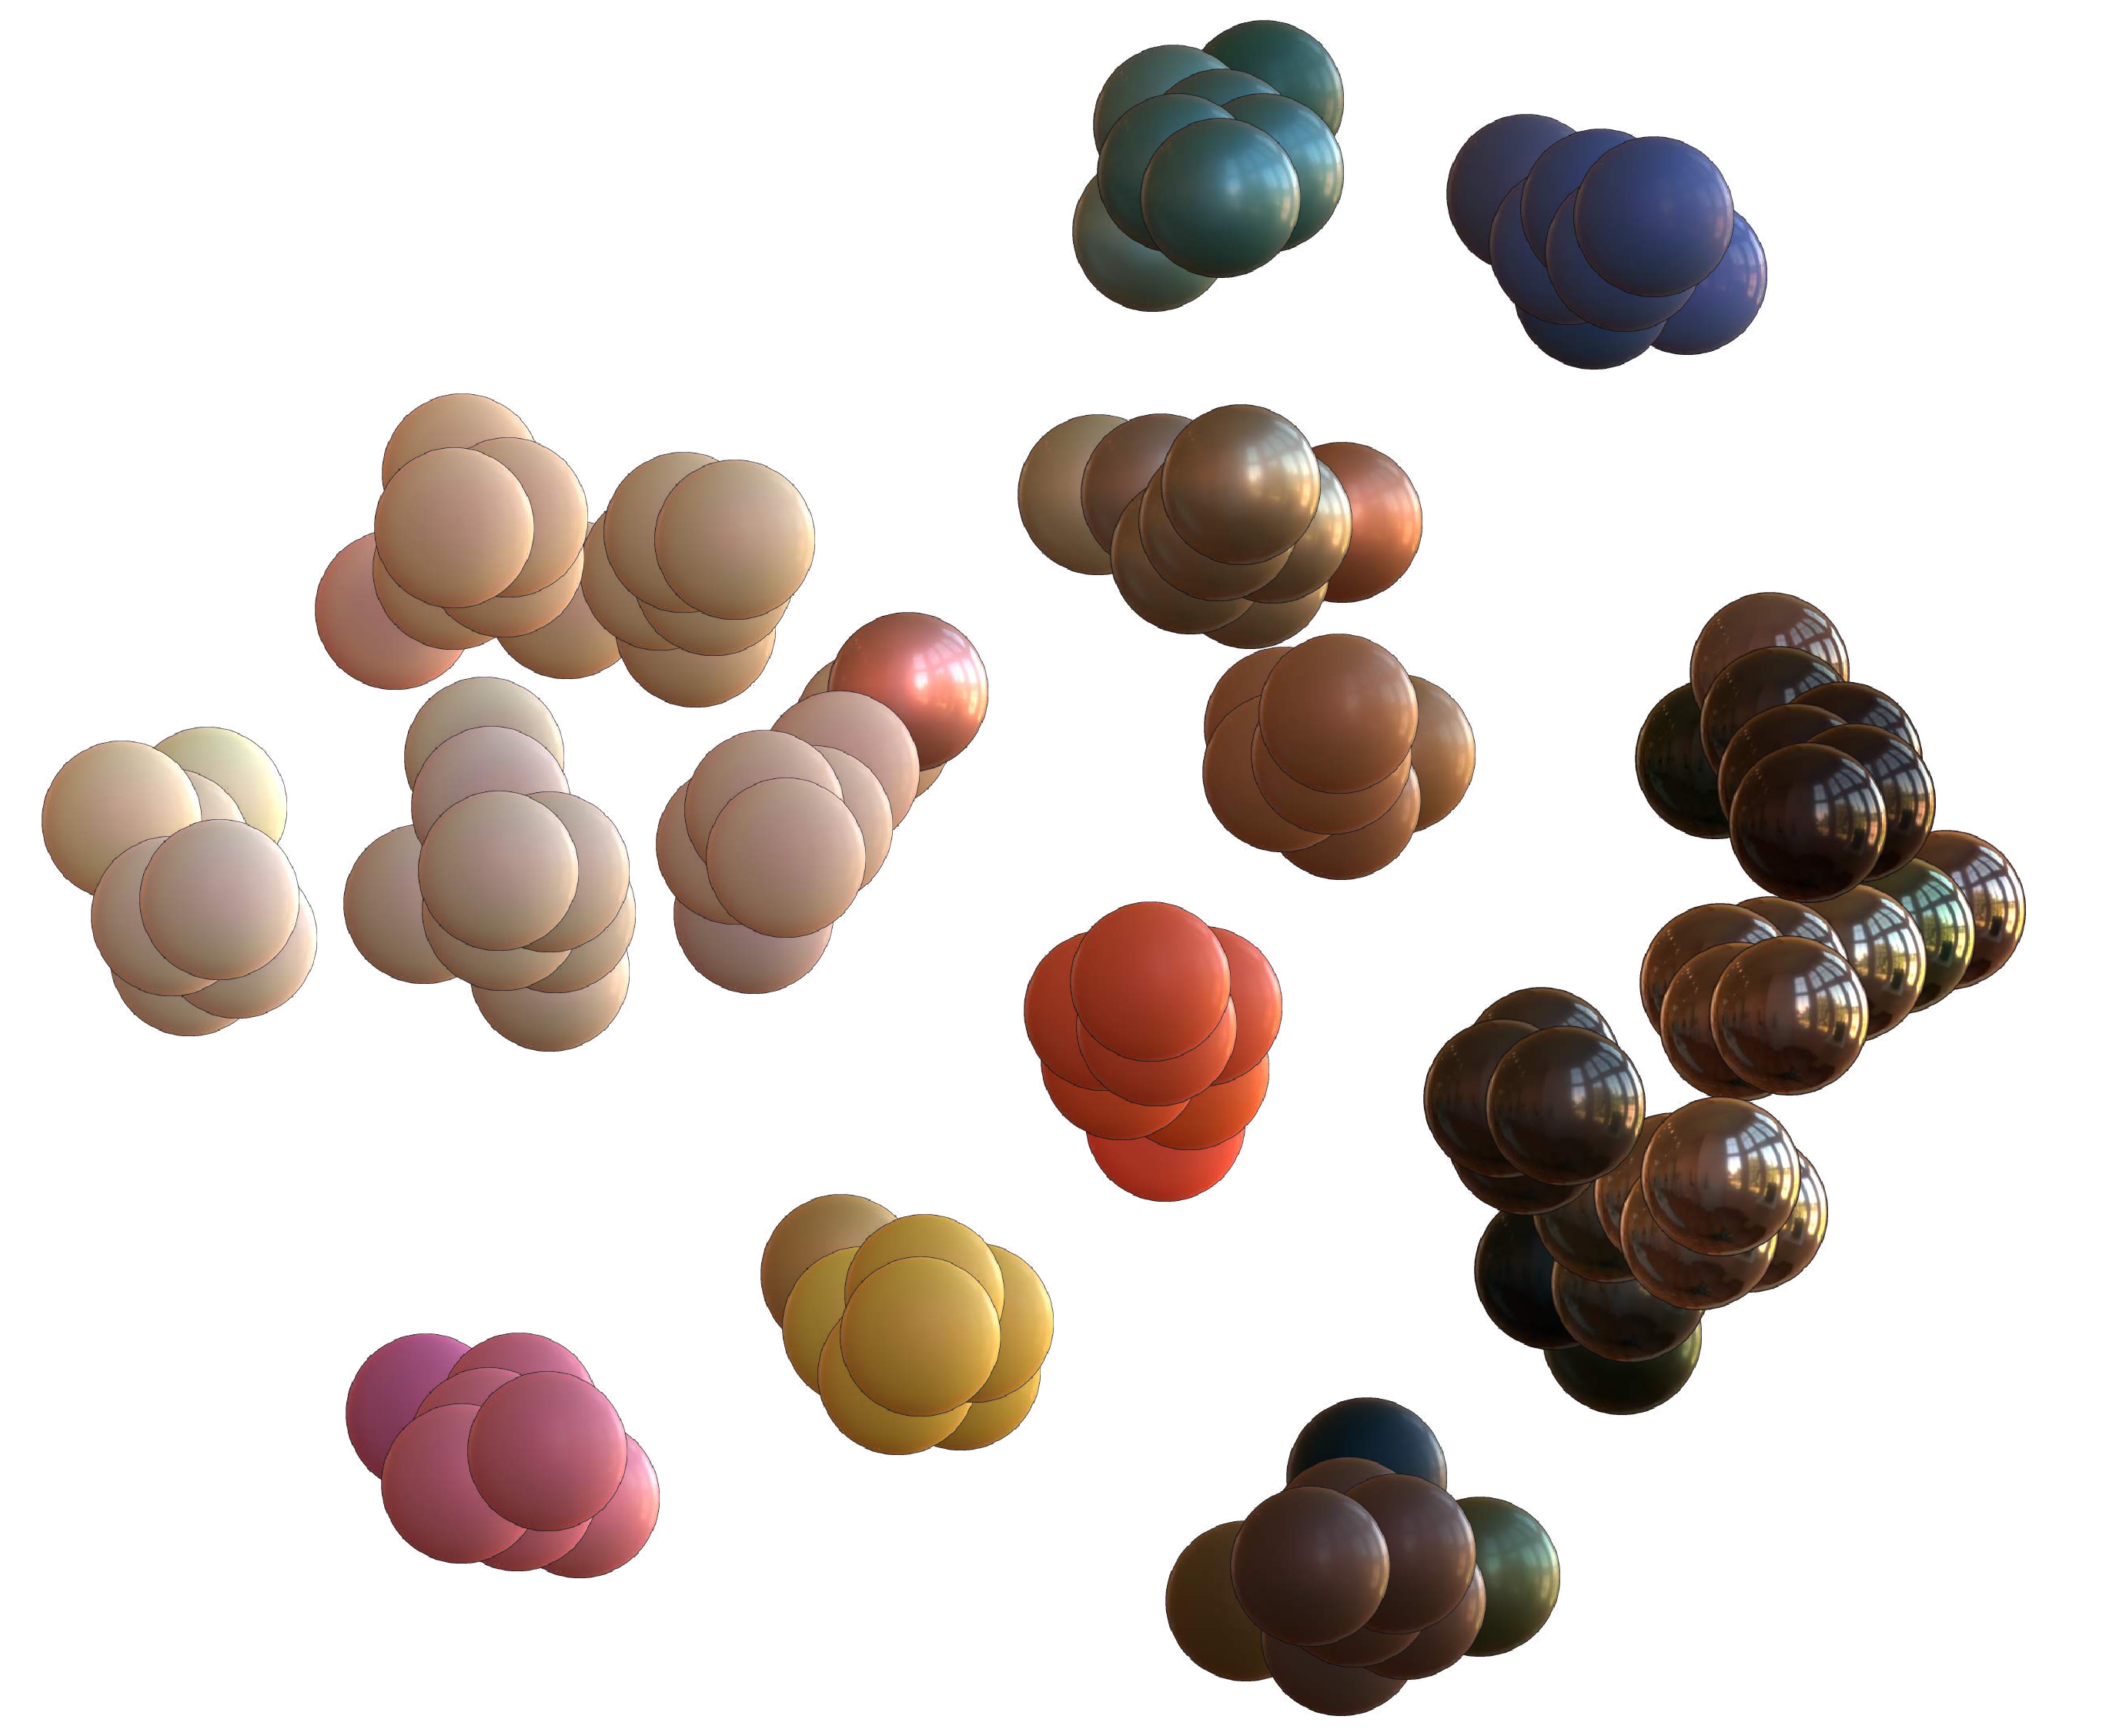
\includegraphics[width=0.8\linewidth]{Chapters/hyperbrdf-figs/tsne6_2_den1-cropped-compressed.pdf}
   \caption{t-SNE clustering of the test embeddings with different sample sizes, including $N=8, 40, 160, 4\,000, 40\,000, 640\,000$.}

   \label{fig:tsne-vis-imputation}
\end{figure}


\subsubsection{Qualitative Comparison}\label{sec:qual_comp}
\begin{figure*}[t]
  \centering
\adjustbox{trim={0.\width} {.\height} {0.89\width} {.\height},clip}%
  {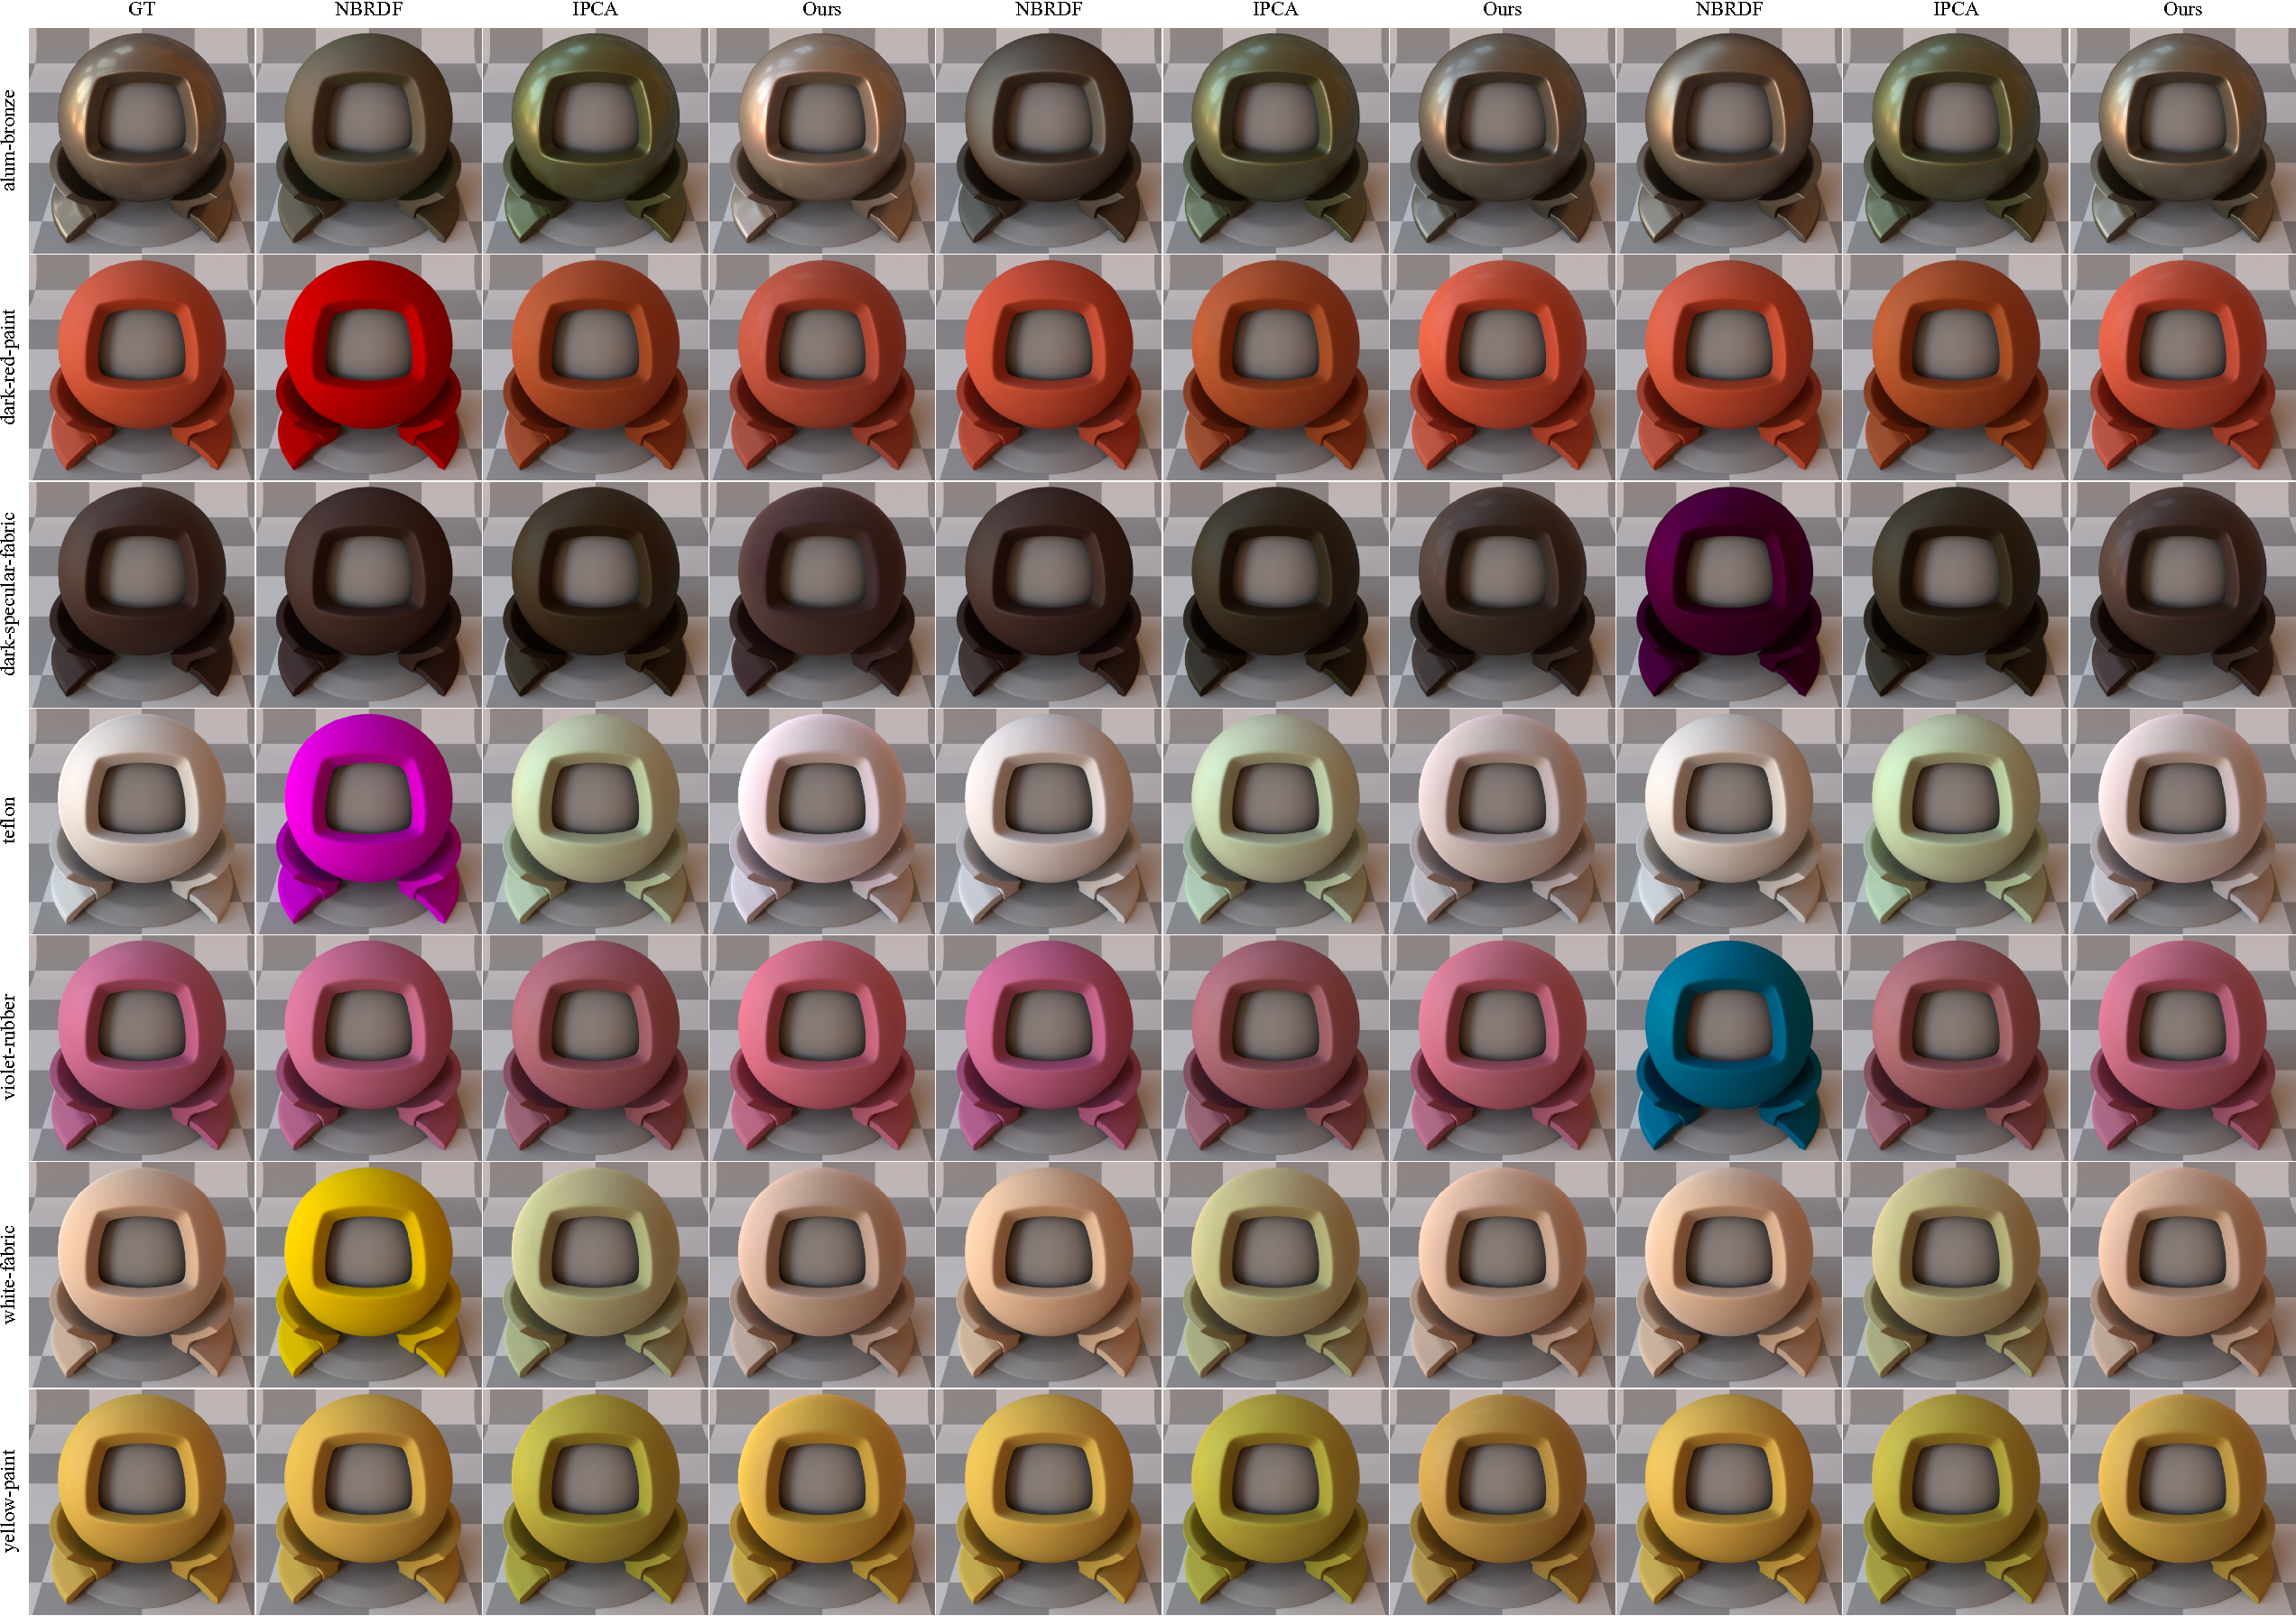
\includegraphics[width=0.9\linewidth]{Chapters/hyperbrdf-figs/imp_comp_upt_3vals.pdf}}
\adjustbox{trim={0.113\width} {.\height} {0.596\width} {.\height},clip}%
  {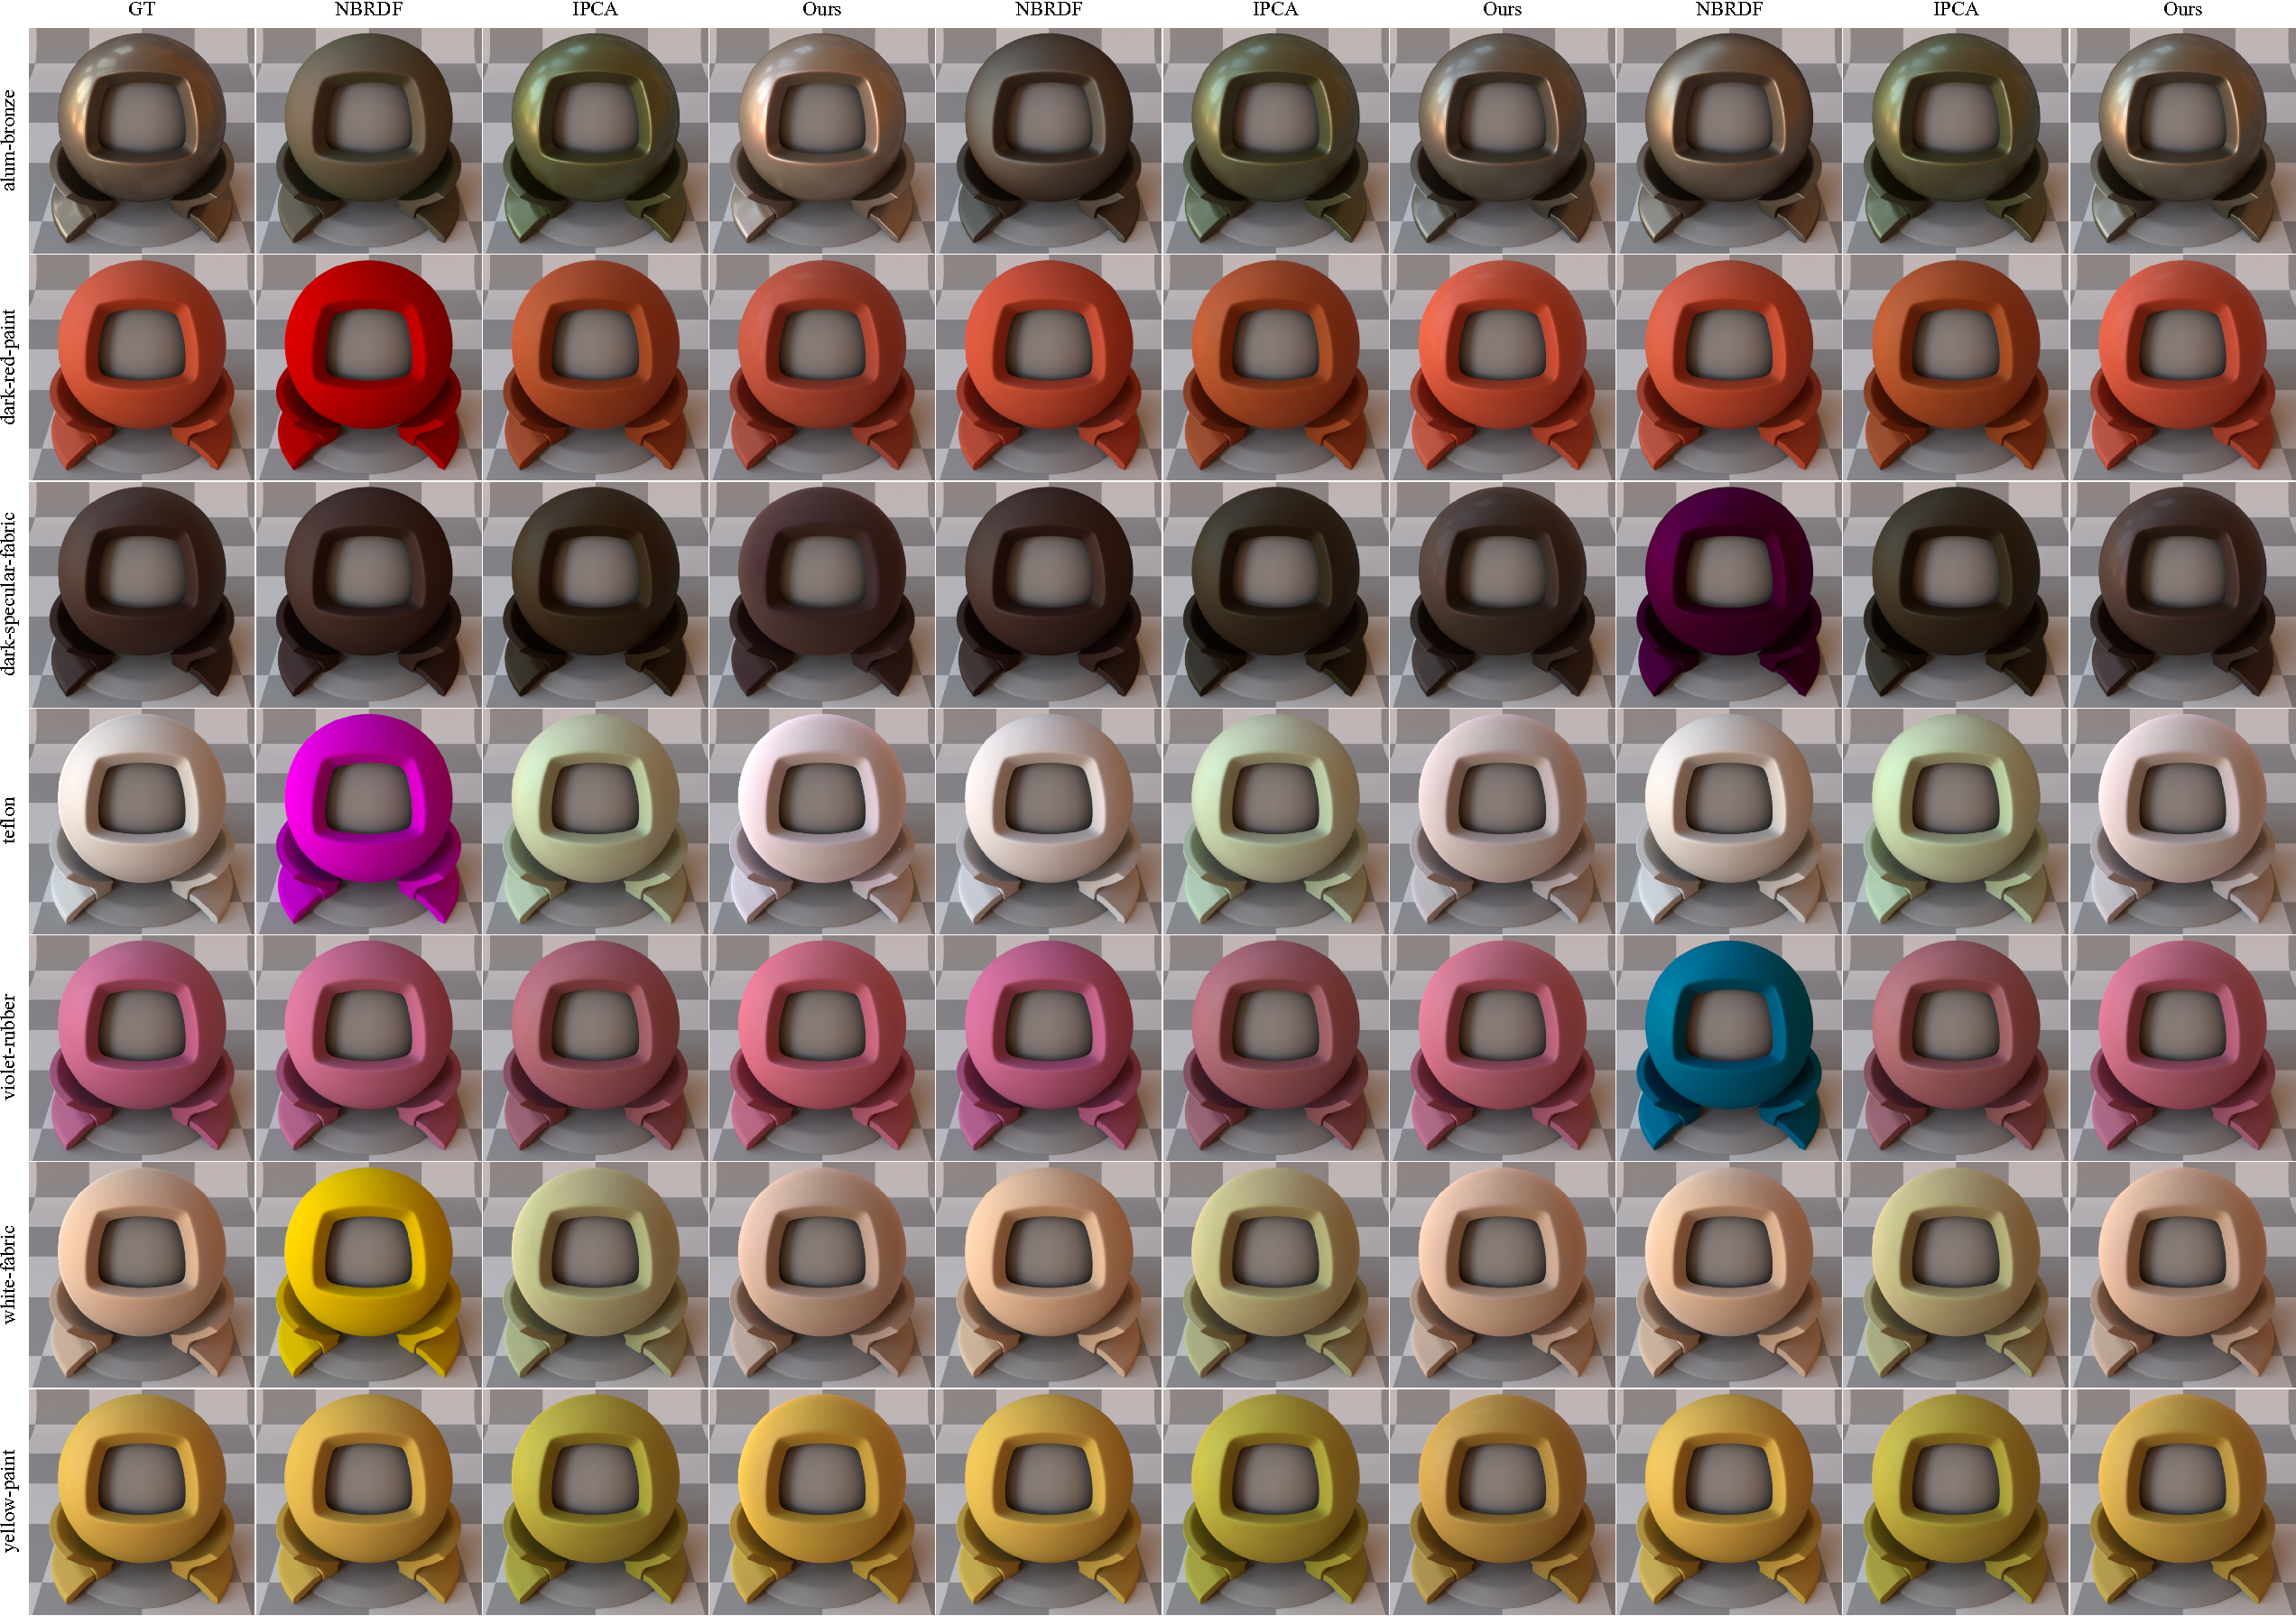
\includegraphics[width=0.9\linewidth]{Chapters/hyperbrdf-figs/imp_comp_upt_3vals.pdf}}
\adjustbox{trim={0.41\width} {.\height} {0.298\width} {.\height},clip}%
  {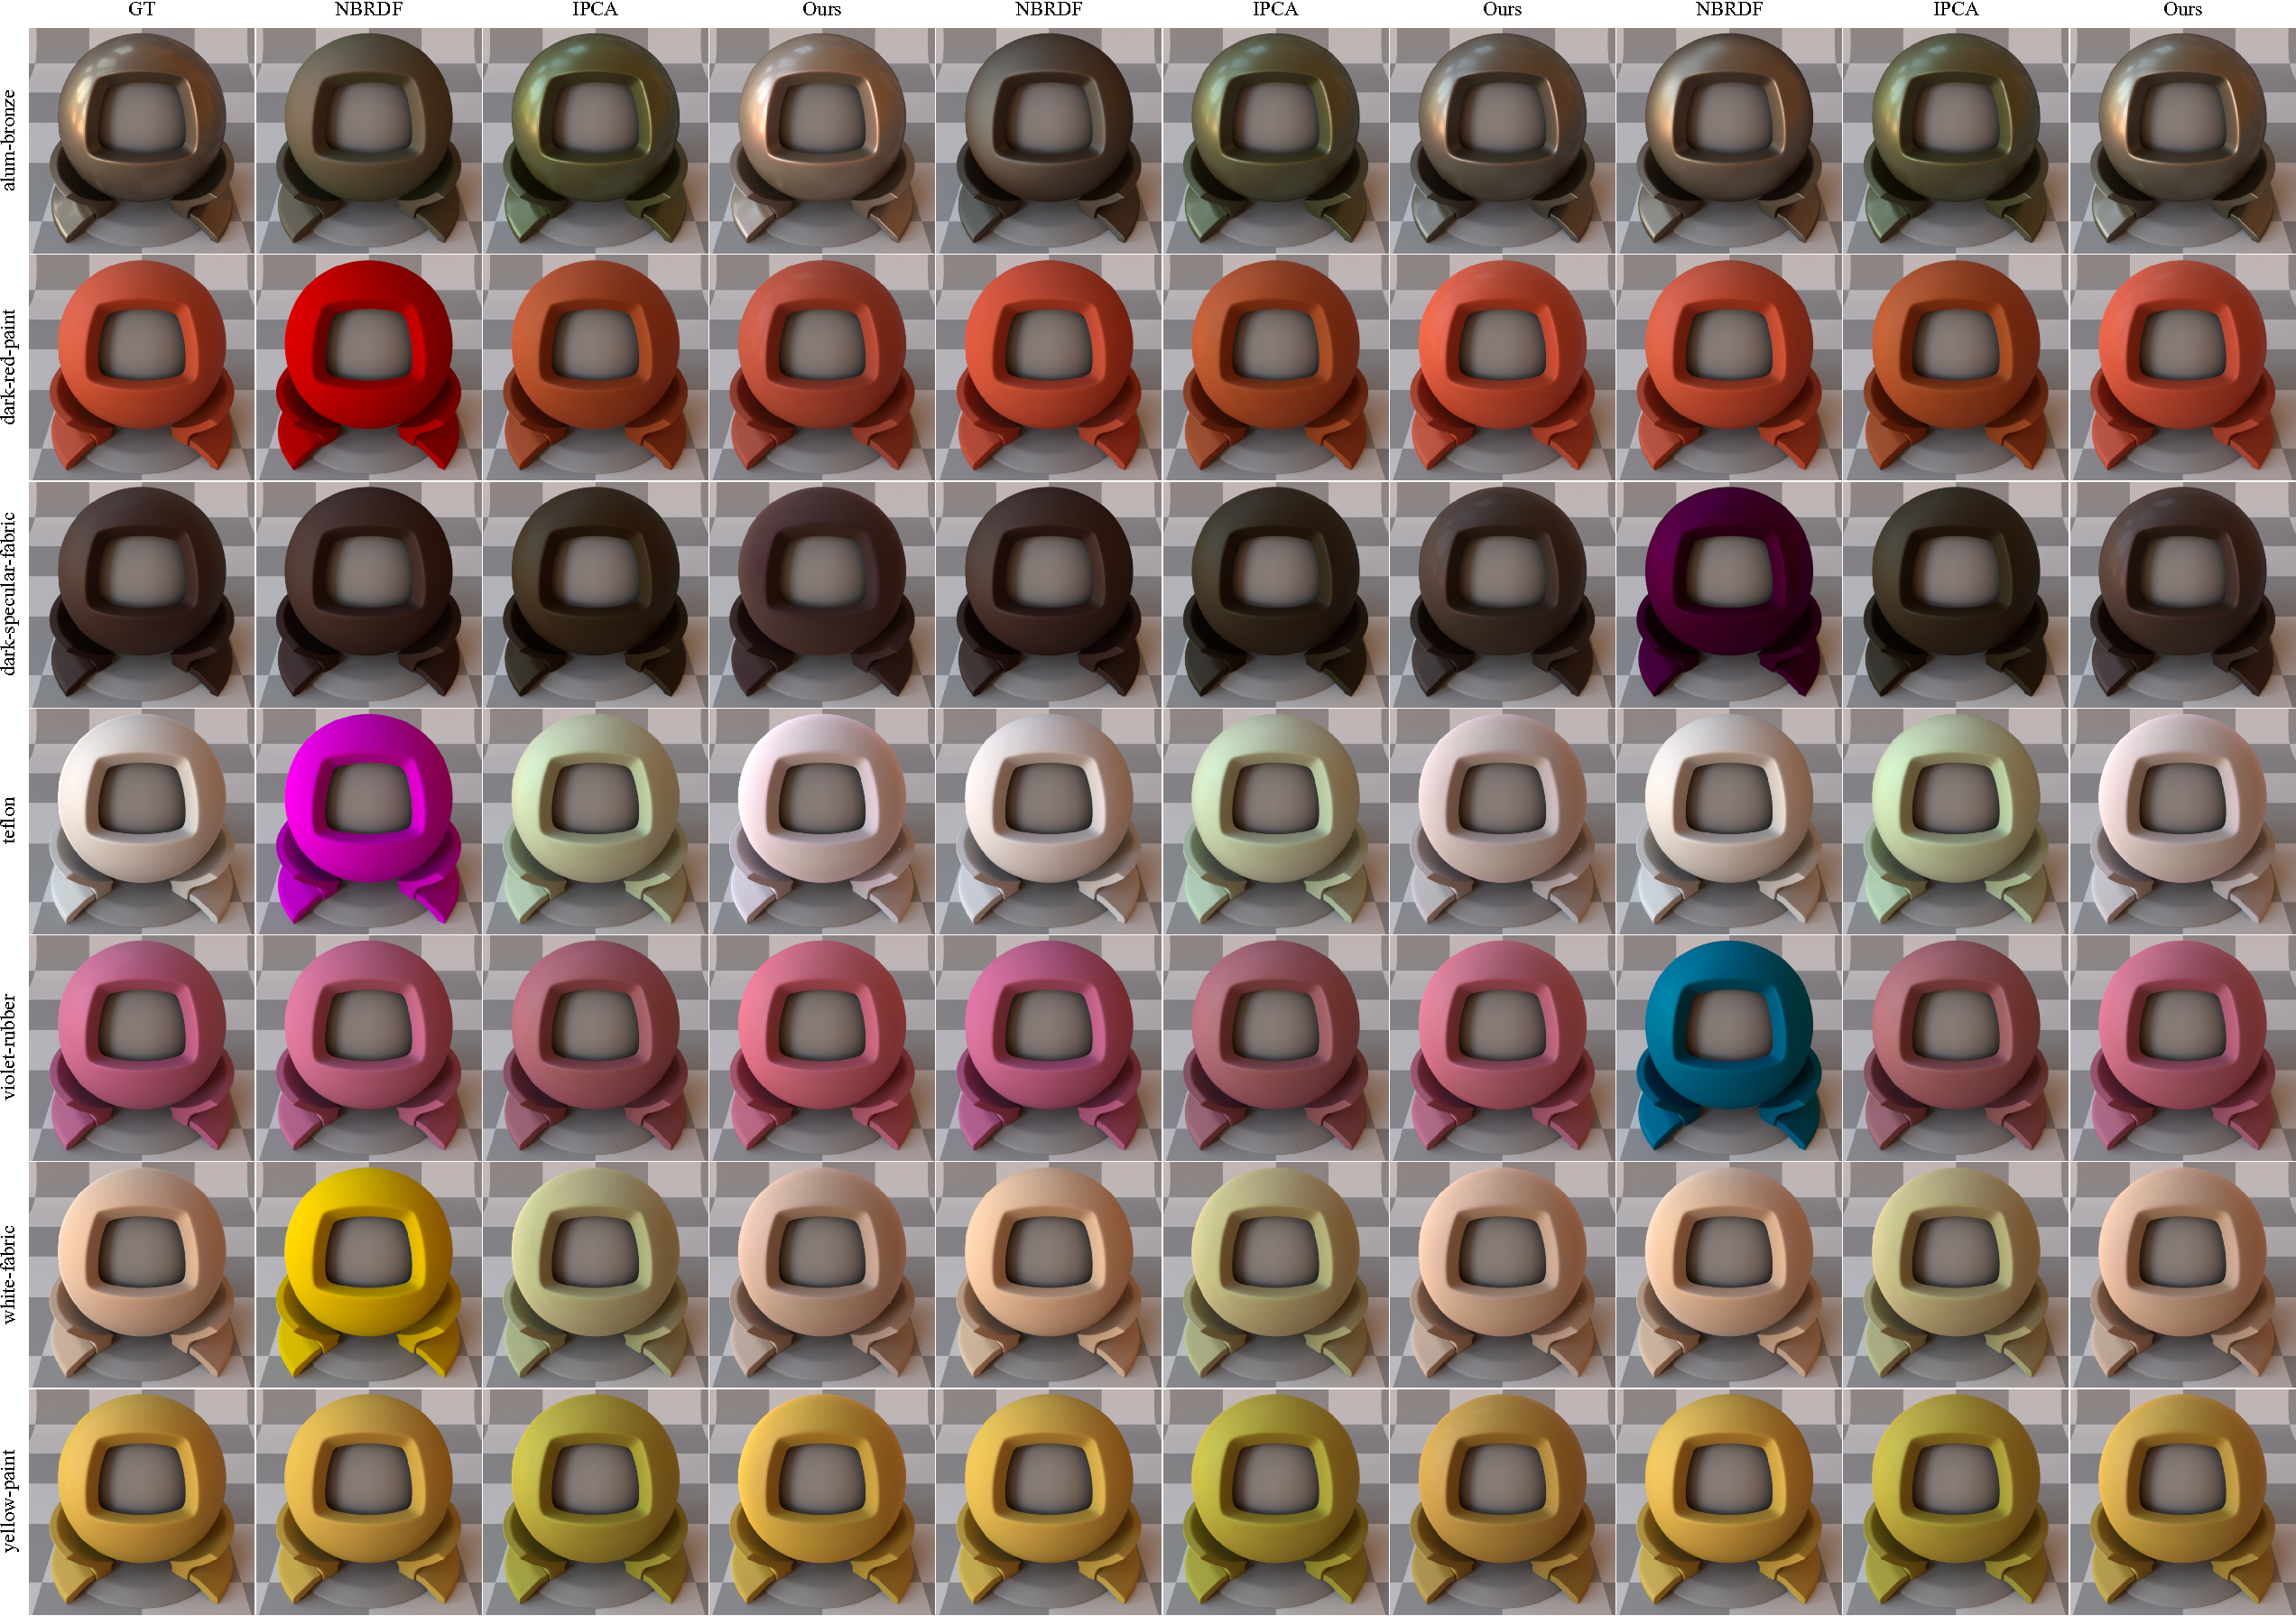
\includegraphics[width=0.9\linewidth]{Chapters/hyperbrdf-figs/imp_comp_upt_3vals.pdf}}
\adjustbox{trim={0.707\width} {.\height} {0.\width} {.\height},clip}%
  {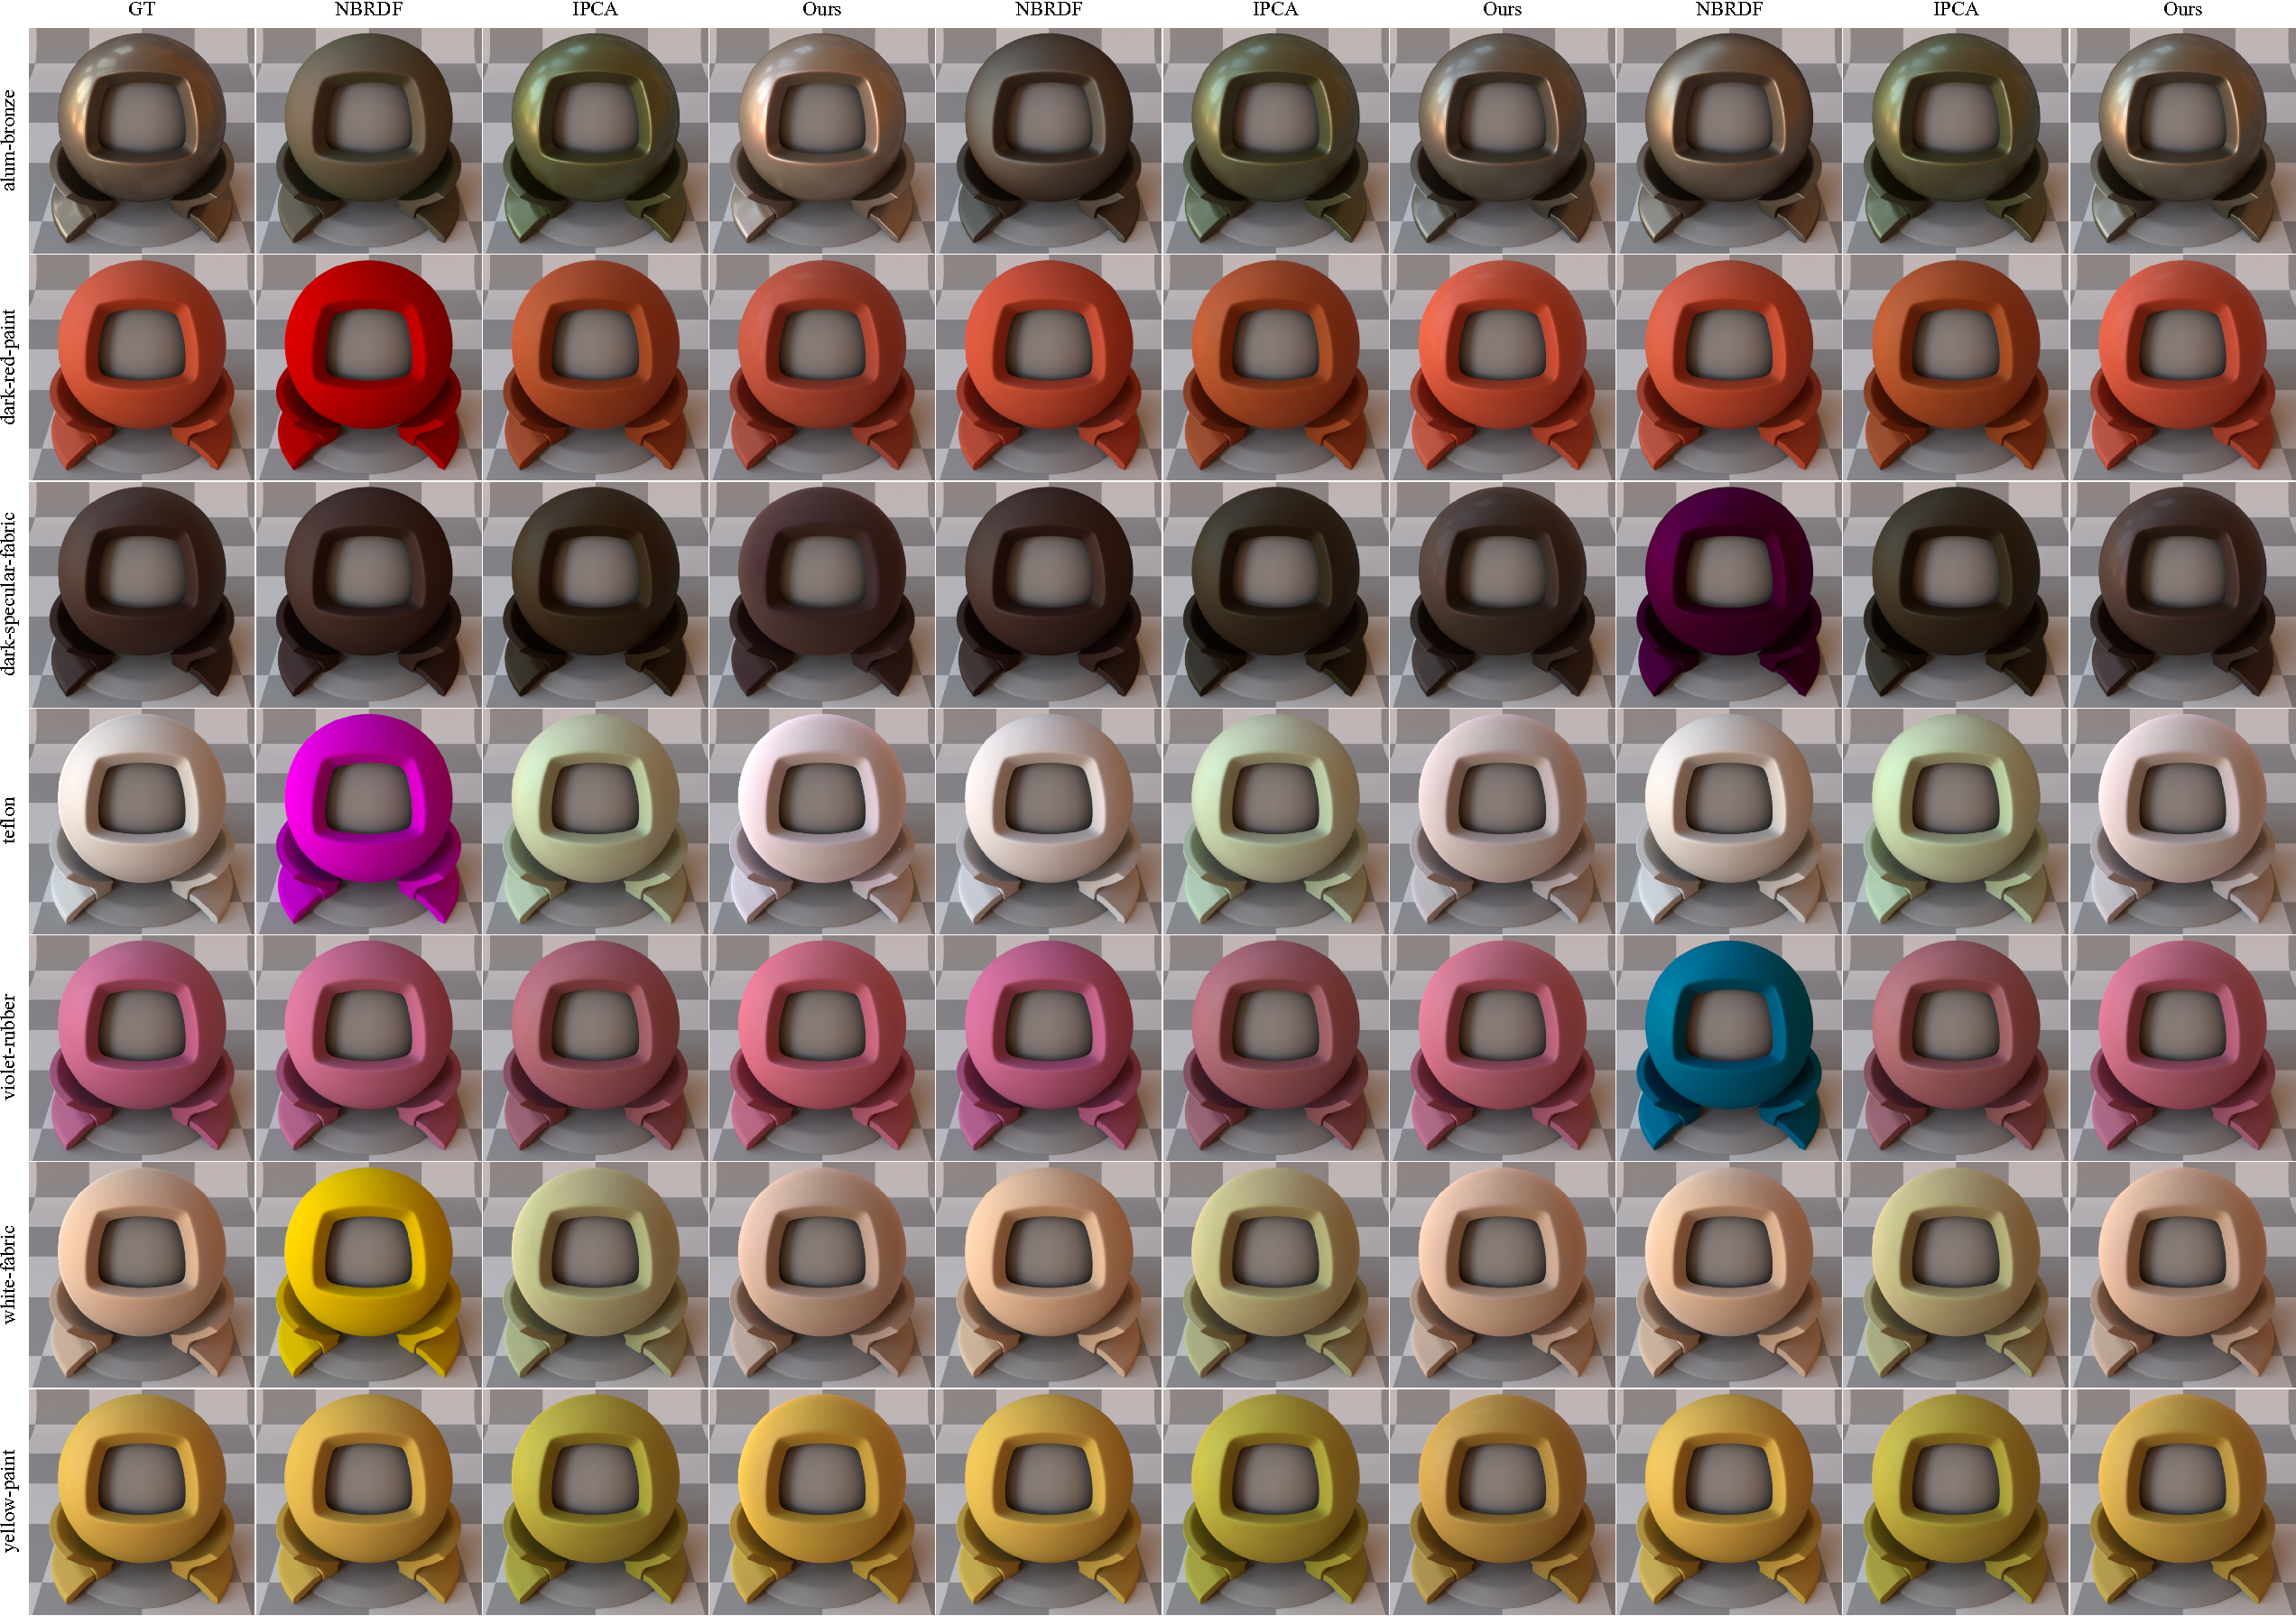
\includegraphics[width=0.9\linewidth]{Chapters/hyperbrdf-figs/imp_comp_upt_3vals.pdf}}

\adjustbox{trim={0.\width} {.\height} {0.89\width} {.06\height},clip}%
  {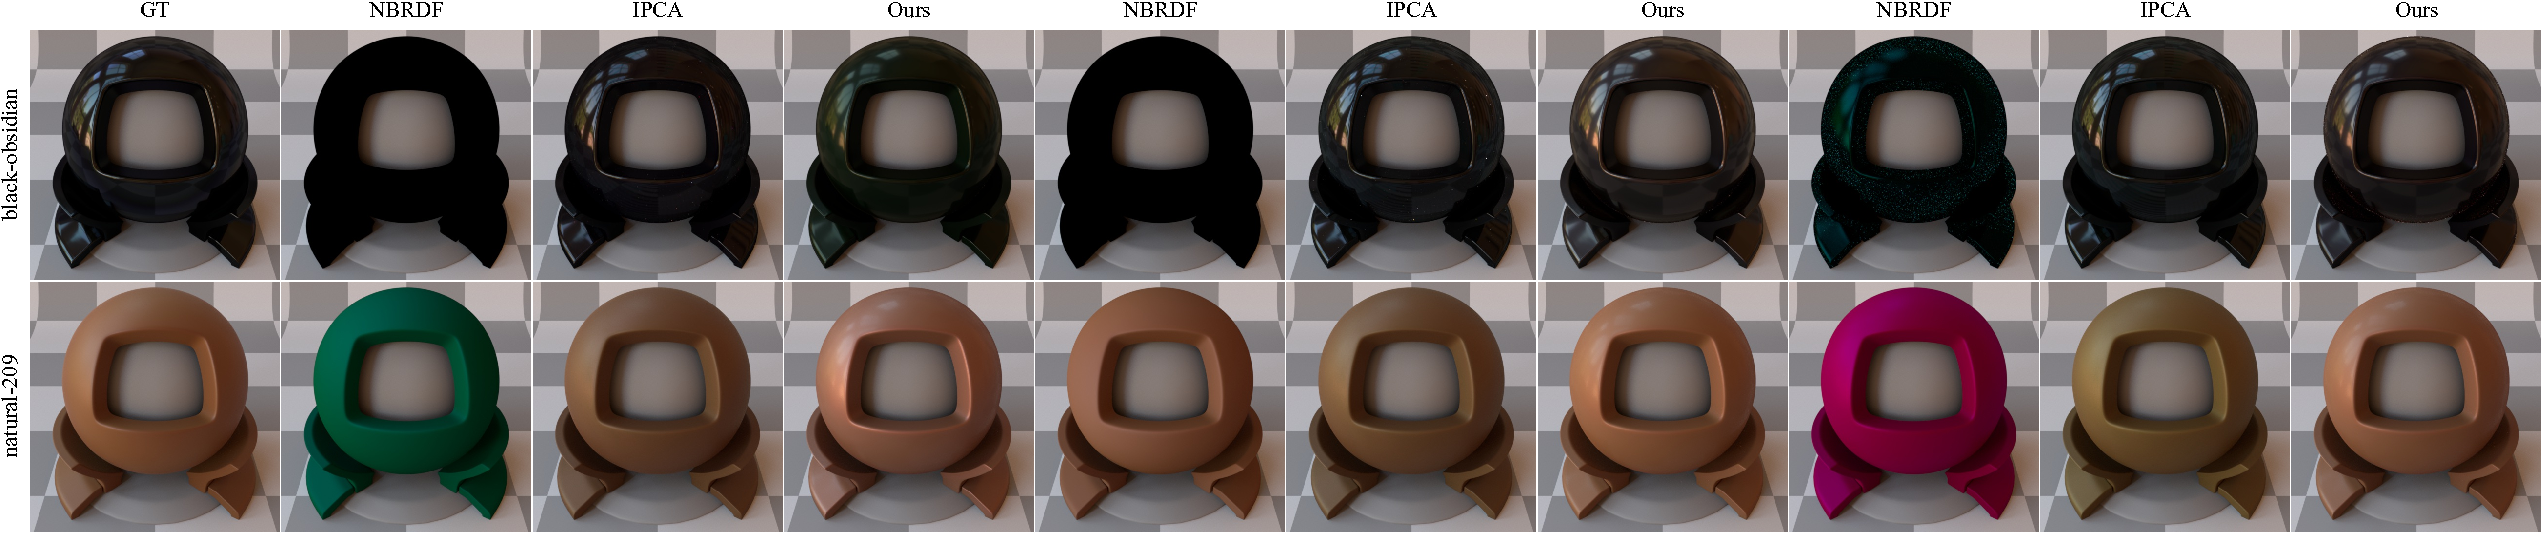
\includegraphics[width=0.9\linewidth]{Chapters/hyperbrdf-figs/imp_comp_upt_3vals_bad.pdf}}
\adjustbox{trim={0.113\width} {.\height} {0.596\width} {.06\height},clip}%
  {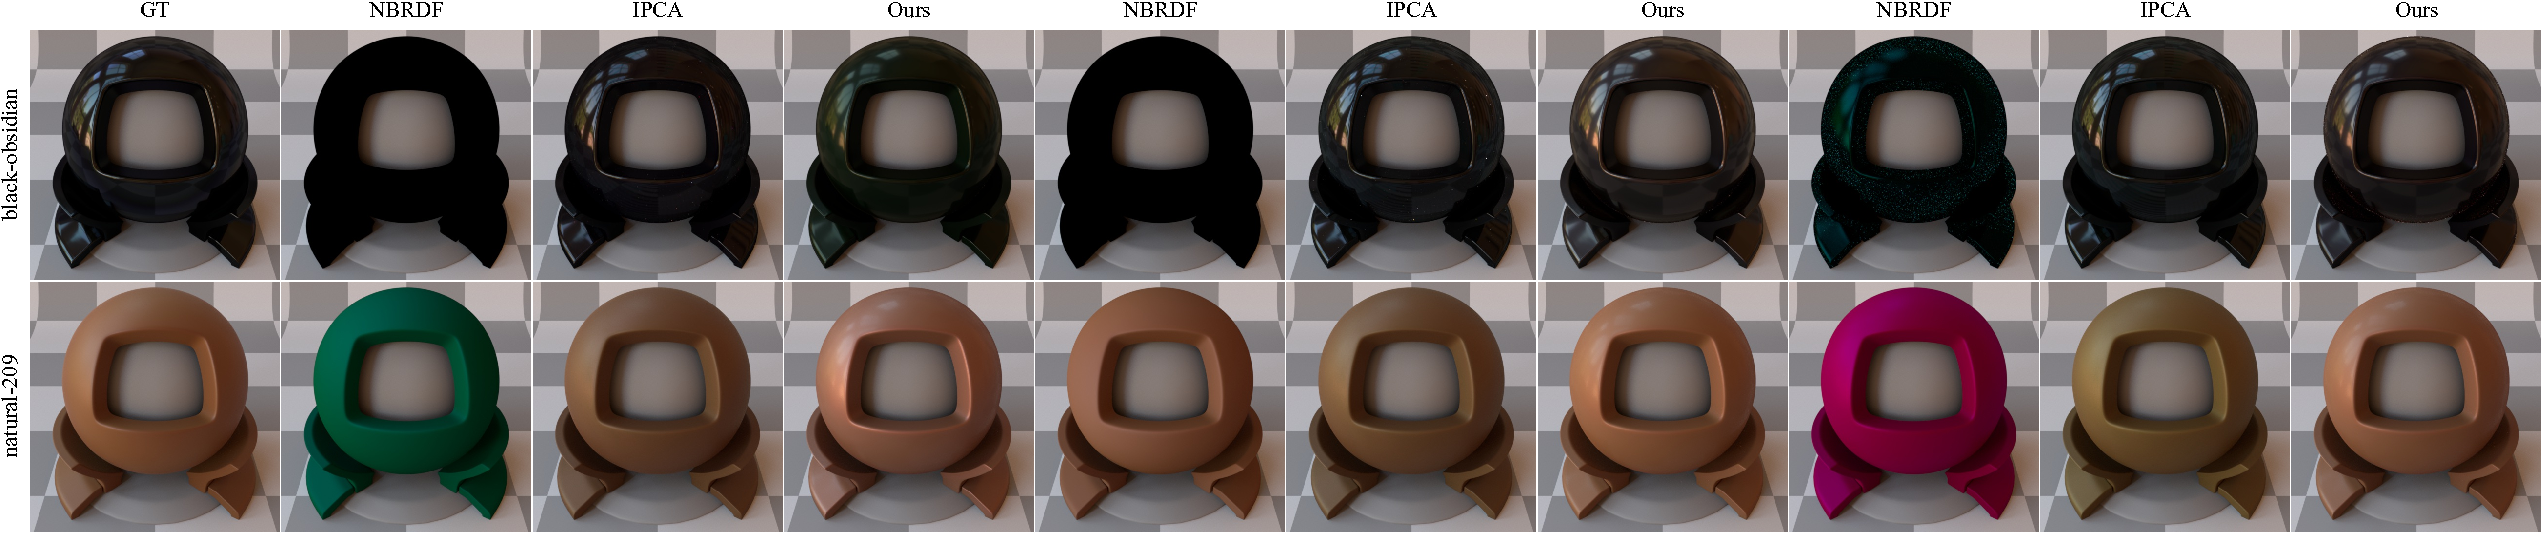
\includegraphics[width=0.9\linewidth]{Chapters/hyperbrdf-figs/imp_comp_upt_3vals_bad.pdf}}
\adjustbox{trim={0.41\width} {.\height} {0.298\width} {.06\height},clip}%
  {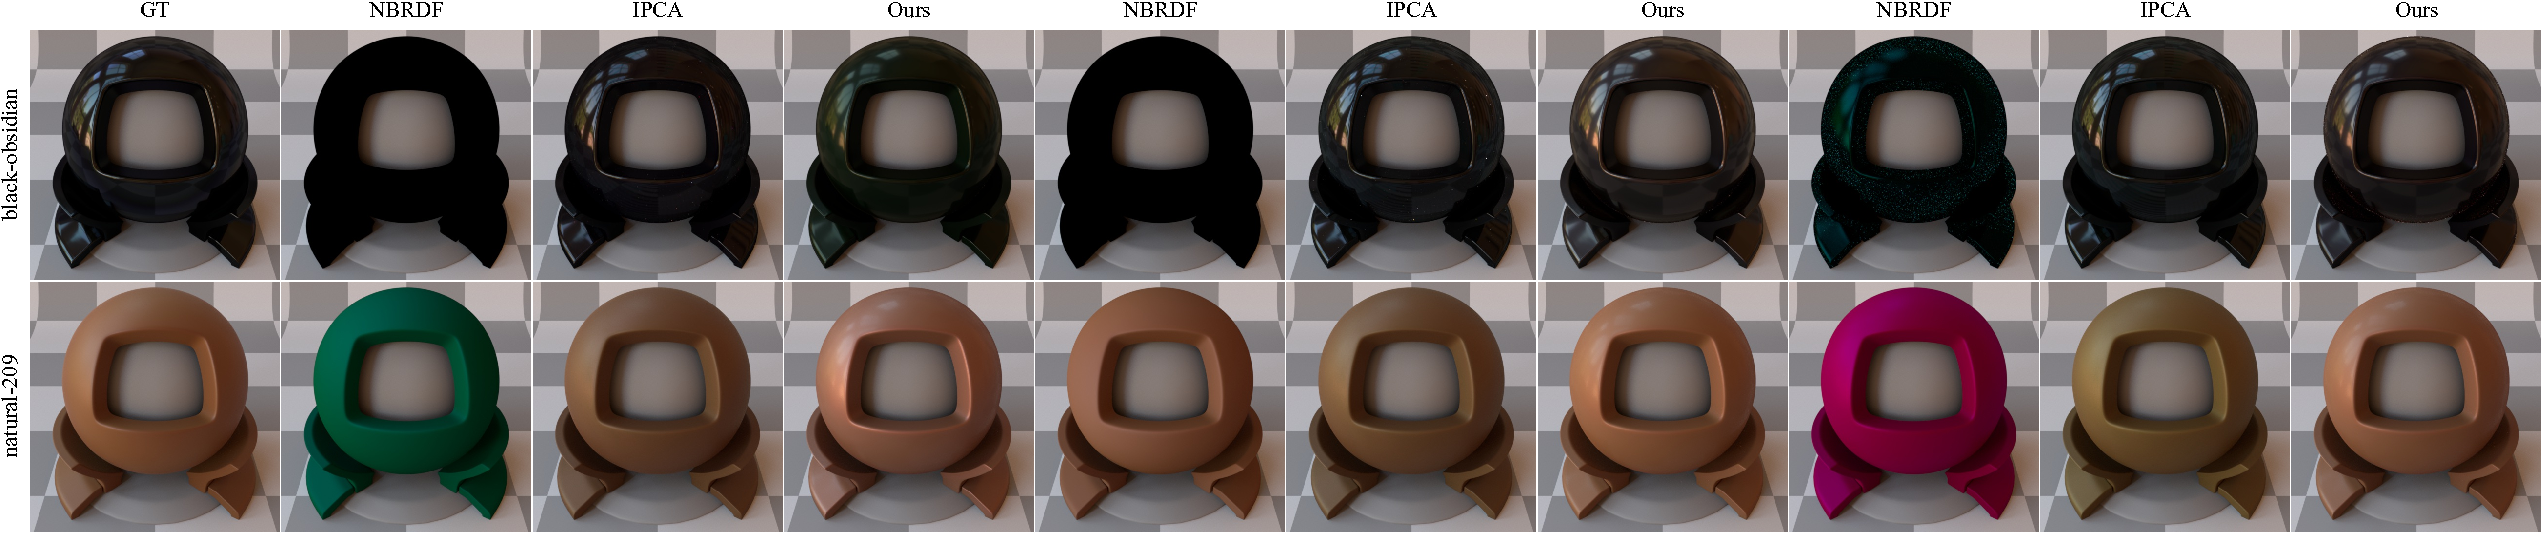
\includegraphics[width=0.9\linewidth]{Chapters/hyperbrdf-figs/imp_comp_upt_3vals_bad.pdf}}
\adjustbox{trim={0.707\width} {.\height} {0.\width} {.06\height},clip}%
  {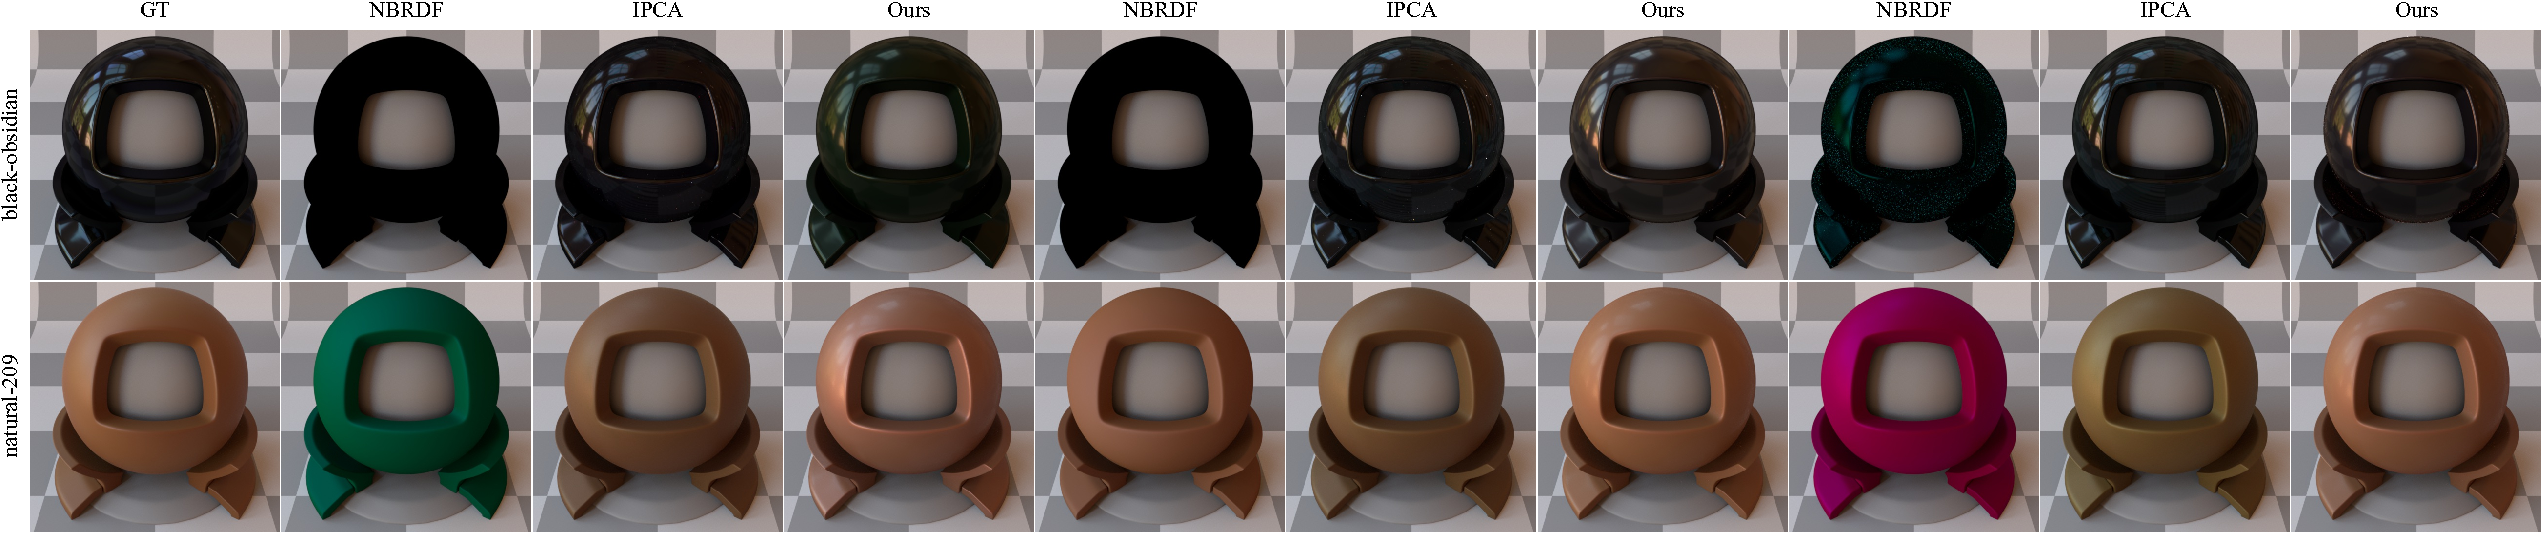
\includegraphics[width=0.9\linewidth]{Chapters/hyperbrdf-figs/imp_comp_upt_3vals_bad.pdf}}
\\
\hspace{1.9cm}{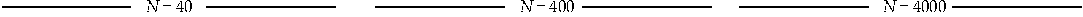
\includegraphics[width=0.8\linewidth]{Chapters/hyperbrdf-figs/N_labels.pdf}}
   \caption{Qualitative comparison results for reconstruction with small sample sizes. Thanks to the prior that our hypernetwork model learns for material appearance through training, it can accurately estimate the BRDFs of unseen materials and preserve the colors better than the baselines.}  

   \label{fig:imp_comp_upt}
\end{figure*}

\begin{figure*}[t]
  \centering
    {
\includegraphics[width=0.35\linewidth]{Chapters/hyperbrdf-figs/legend.png}}\\
  {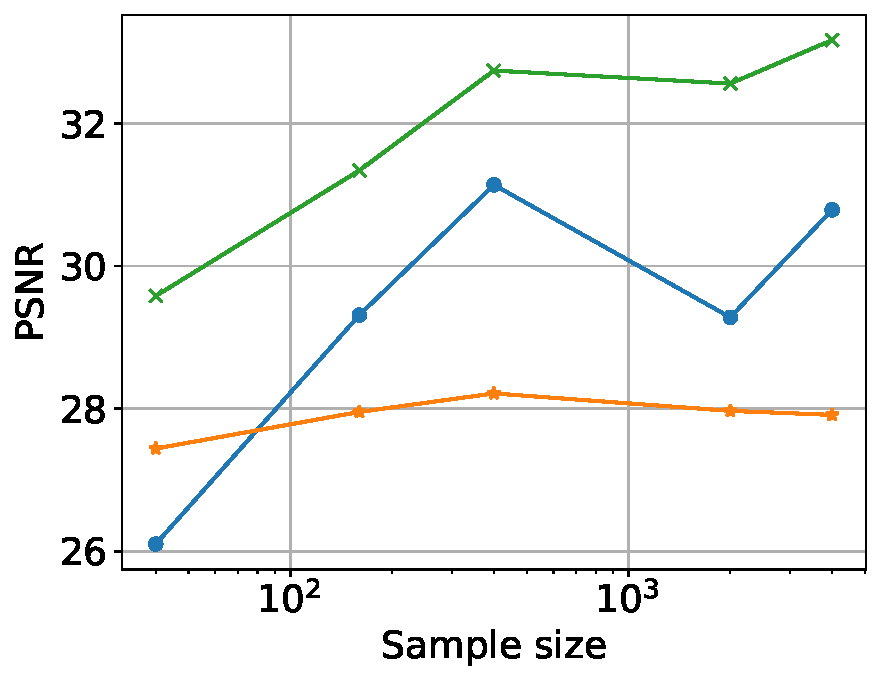
\includegraphics[width=0.32\linewidth]{Chapters/hyperbrdf-figs/PSNR.pdf}}
  {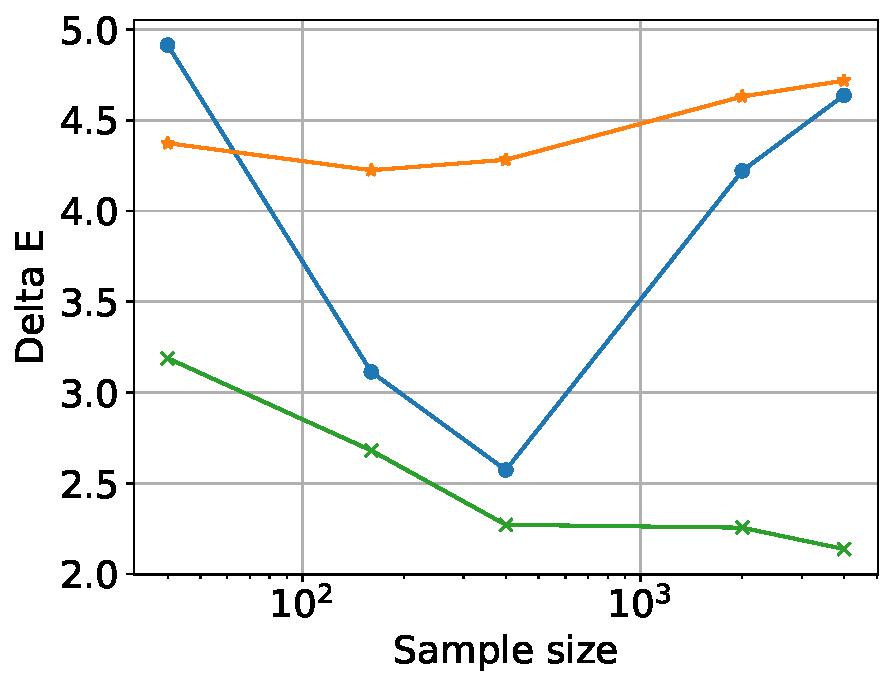
\includegraphics[width=0.32\linewidth]{Chapters/hyperbrdf-figs/DeltaE.pdf}}
  \adjustbox{trim={0.\width} {.0\height} {0.\width} {.\height},clip}%
    {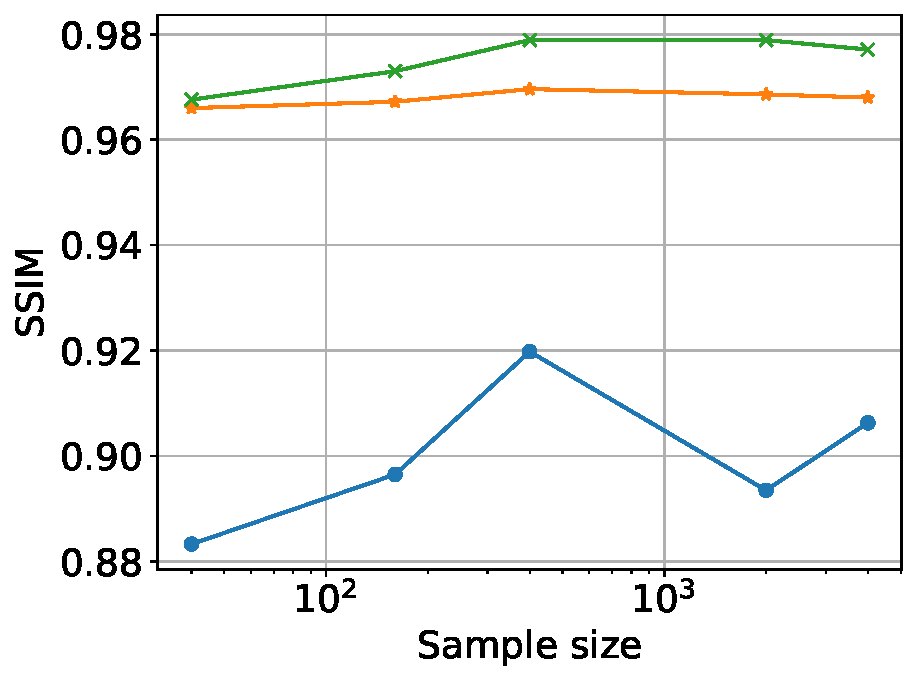
\includegraphics[width=0.32\linewidth]{Chapters/hyperbrdf-figs/SSIM.pdf}}
   \caption{Average PSNR, Delta E (CIE 2000), and SSIM results across different sample sizes. }
   \label{fig:imp_plots}
\end{figure*}



We first compare our results with the ground truth renderings for varying sample sizes. Figure \ref{fig:imp_comp_upt} shows that the hypernetwork can still reconstruct test materials even with $N = 40$ samples. However, as we reduce the sample number to 10, the reconstruction quality highly decreases. For additional results with different query sample sizes, please refer to our supplementary.


During inference time, hypernetwork fits the samples to a BRDF. Even with a few samples, it can still accurately reconstruct test materials. Its success comes from the fact that it learns a prior for material appearance through training with a dataset of multiple materials. Therefore, we validate our generalizable approach by comparing the hypernetwork with NBRDF \cite{sztrajman2021neural} and PCA with Log Relative Mapping (IPCA) \cite{nielsen2015optimal}.


NBRDF \cite{sztrajman2021neural} is designed to implicitly represent an individual BRDF. It can reconstruct materials with very high accuracy (Structural Similarity Index of around 0.995) when the sample size is high. It first trains the network on a material and then estimates the BRDF values of the same material. For a fair comparison, we first fit an NBRDF model to a material BRDF with the query sample size, then estimate the function with the same sample size. 

We also compare our results with a PCA-based strategy (IPCA). To represent the BRDF data, PCA-based methods  \cite{matusik2003data, ngan2006image} construct a matrix ${A} \in \mathbb{R}^{m \times n}$, where n = 180 × 90 × 90 × 3 = $4\,374\,000$ is the feature number, m = 80 is sample number. The matrix is later decomposed into its principal components via Singular Value Decomposition. PCA itself struggles with the decomposition of high dynamic range data. Therefore, the Log Relative Mapping (IPCA) is proposed~\cite{nielsen2015optimal}, which is defined in our pre-processing step (Section \ref{sec:pre-proc}). This improves the reconstruction qulity, offering competitive reconstructions against our method as shown in Figure \ref{fig:imp_comp_upt}.


For all methods including ours, samples are drawn from a uniform distribution over Rusinkiewicz coordinates. For IPCA results, we split train and test dataset in the same way as ours, i.e., 80 MERL materials for train and 20 for test, and use all available samples for learning the principal components. To reconstruct the test materials from sparse samples, we first run a least-squared-error optimization and predict the weights of the material for the corresponding principal components. To decide the number of components, we ran an additional ablation study, where 
we computed the average mean squared error over the test dataset for the reconstruction from sparse samples ($N = 40$). We observed that ($N_{PC} = 8$) gives the minimum error on the test dataset. Hence, we choose the number of principal components as $N_{PC} = 8$ and keep it same for sparse sampling results.

 
We keep the range for sparse sample numbers between $N = 40$ and $N = 4000$. Figure \ref{fig:imp_comp_upt} shows the rendering results for the minimum and maximum number of our range. Compared to both IPCA and NBRDF, our hypernetwork can capture the appearances more precisely. Although our approach has difficulty estimating specular components (last two rows in Figure~\ref{fig:imp_comp_upt}), overall it offers reconstructions with much higher accuracy.

We observe that the diffuse colors of some reconstructed materials by NBRDF can be completely off (natural-209, teflon) due to function fitting with sparse samples. Hypernetwork, on the other hand, can preserve diffuse colors better thanks to the prior it learns through training.


\subsubsection{Quantitative Evaluation}

We compare our method quantitatively with the aforementioned techniques in multiple image-based error metrics through rendering results. The metrics include peak signal-to-noise ratio (PSNR), Delta E (CIE 2000), and structural similarity index (SSIM). We take the average over the test dataset for each metric. We plot the metric results across five different sample sizes (40, 160, 400, 2000, 4000). Since we optimize IPCA on the test dataset for the $N = 40$ case, it offers more competitive results. Nevertheless, our method can reconstruct the BRDFs of unseen materials more precisely. Figure \ref{fig:imp_plots} shows that across all sample sizes, the hypernetwork attains superior performance in terms of PSNR, Delta E (CIE 2000) and SSIM. 

Additionally, Table \ref{table: ours_diff_samples} shows that expanding the training set, even with materials captured from a different point-based setup, helps improve the performance of the hypernetwork. Also, note that compared to MERL materials, the colors of RGL materials are more saturated, which could explain a slight increase in Delta E.


 \begin{table*}
    \centering
    \caption{Hypernetwork sparse reconstruction - Average metric results across varying sample sizes ($N$) over the test set. We highlight \colorbox{blue!25}{best} and \colorbox{orange!25}{second best} results.}
    
    {\begin{tabular}{l@{\hskip 0.4in}c@{\hskip 0.2in}c@{\hskip 0.2in}c@{\hskip 0.1in}|@{\hskip 0.1in}c@{\hskip 0.2in}c@{\hskip 0.2in}c}\toprule
    

& \multicolumn{3}{c}{MERL} & \multicolumn{3}{c}{MERL + RGL}
\\\cmidrule(lr){2-4}\cmidrule(lr){5-7}
% \toprule
  $N$ & PSNR\textuparrow & Delta E\textdownarrow & SSIM\textuparrow & PSNR\textuparrow & Delta E\textdownarrow & SSIM\textuparrow \\

 \toprule

$40$ & 29.581 & 3.189 & 0.968 & 30.018 & 3.112 & 0.963\\
$160$ & 31.341 & 2.681 & 0.973 & 31.929 & 2.454 & 0.962\\
$400$ & 32.743 & 2.272 & \cellcolor{blue!25} 0.979 & 33.855 & 2.432 & 0.977\\
$2000$ & \cellcolor{blue!25} 34.527 & \cellcolor{orange!25}2.256 & \cellcolor{blue!25} 0.979 & \cellcolor{blue!25} 34.527 & \cellcolor{orange!25} 2.243 & \cellcolor{blue!25} 0.983\\
$4000$ & \cellcolor{orange!25} 33.170 &  \cellcolor{blue!25} 2.138 & \cellcolor{orange!25} 0.977 & \cellcolor{orange!25} 34.355 & \cellcolor{blue!25} 2.166 & \cellcolor{orange!25} 0.982\\

\bottomrule
    \end{tabular}\par}
    \label{table: ours_diff_samples}
\end{table*}

\subsection{Compression}\label{sec:compression}
The high capacity of the hypernetwork also allows the compression of the densely sampled BRDF data into low-dimensional latent representations. The hypernetwork can process highly compact BRDF embeddings, and once decoded, reconstructs the BRDF data precisely. We compare our method with Neural Processes (NPs) \cite{zheng2021compact}, the state-of-the-art BRDF compression method, and show that our hypernetwork model overall performs better in all three metrics. 


To compare our method with NPs, we overfit our model to the mixed dataset of MERL and isotropic RGL materials, consisting of 151 materials in total. Since the latent dimension of NPs is 7D, we also train our network with 7D latent space. It is worth mentioning that NPs cause 
invalid sample values in certain MERL materials, blacking some parts of the renderings. In contrast, our method consistently decompresses materials with high reconstruction accuracy; see Table \ref{table: oursvsnps}. Rendering results can be found in our supplementary (Compression.pdf).

\begin{table}
    \centering
    \caption{Compression - Average metric results over the renderings of the entire MERL dataset. We highlight \colorbox{blue!25}{best} and \colorbox{orange!25}{second best} results.}

    {%
    {\begin{tabular}{l@{\hskip 0.5in}c@{\hskip 0.3in}c@{\hskip 0.3in}c}\toprule


  &  PSNR \textuparrow & Delta E \textdownarrow & SSIM \textuparrow \\
 \toprule
 Ours (40D) & \cellcolor{blue!25} 47.682 & \cellcolor{blue!25} 0.567 & \cellcolor{blue!25} 0.994\\
 Ours (7D) & \cellcolor{orange!25} 47.492 & \cellcolor{orange!25} 0.574 & \cellcolor{blue!25} 0.994\\
 NPs & 46.125 & 2.424 & 0.935\\
 IPCA & 29.892 & 3.315 & 0.979\\

\bottomrule
    \end{tabular}\par}}
    \label{table: oursvsnps}
\end{table}


\begin{figure*}[ht]
  \centering
  {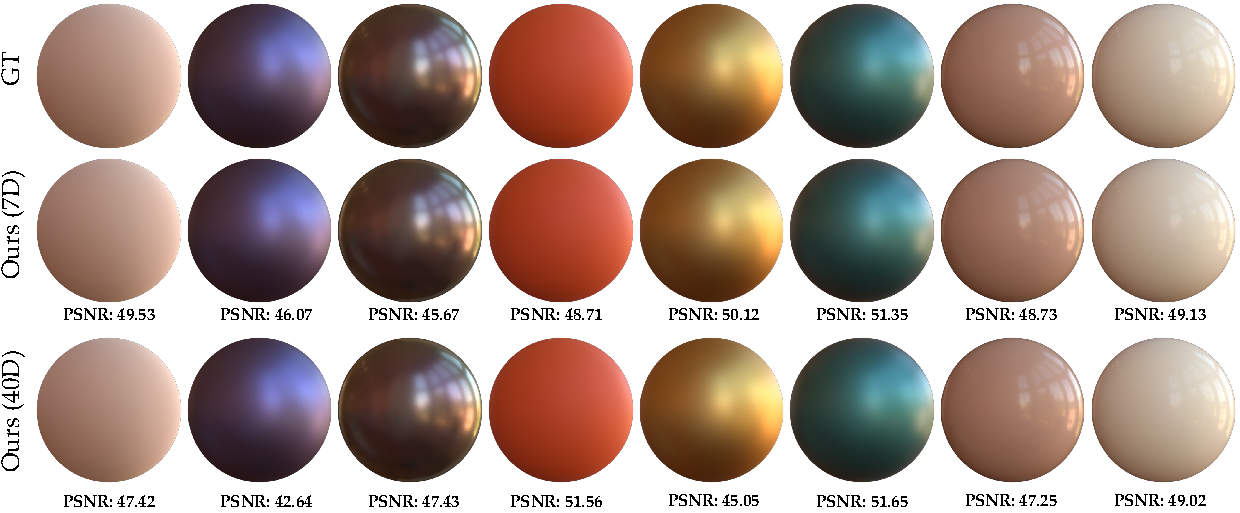
\includegraphics[width=0.9\linewidth]{Chapters/hyperbrdf-figs/compression_comp.pdf}}
   \caption{Reconstruction results for BRDF compression (GT: ground truths).}
   \label{fig:comp-fig}
\end{figure*}


\subsection{BRDF Editing}

Compared to analytic BRDFs that have a fixed number of parameters to tweak, editing measured BRDFs is rather a nontrivial task due to irregular data structure. On the other hand, our network is capable of BRDF editing thanks to its representation of materials in a low-dimensional space. We can easily reconstruct various appearances by linearly interpolating between the embeddings of two different materials. Figure \ref{fig:interpolation} shows newly-reconstructed materials through linear interpolation between two different embeddings from the reconstructed MERL materials. 


\begin{figure*}[ht]
  \centering
  % \fbox{\rule{0pt}{2in} \rule{0.9\linewidth}{0pt}}
   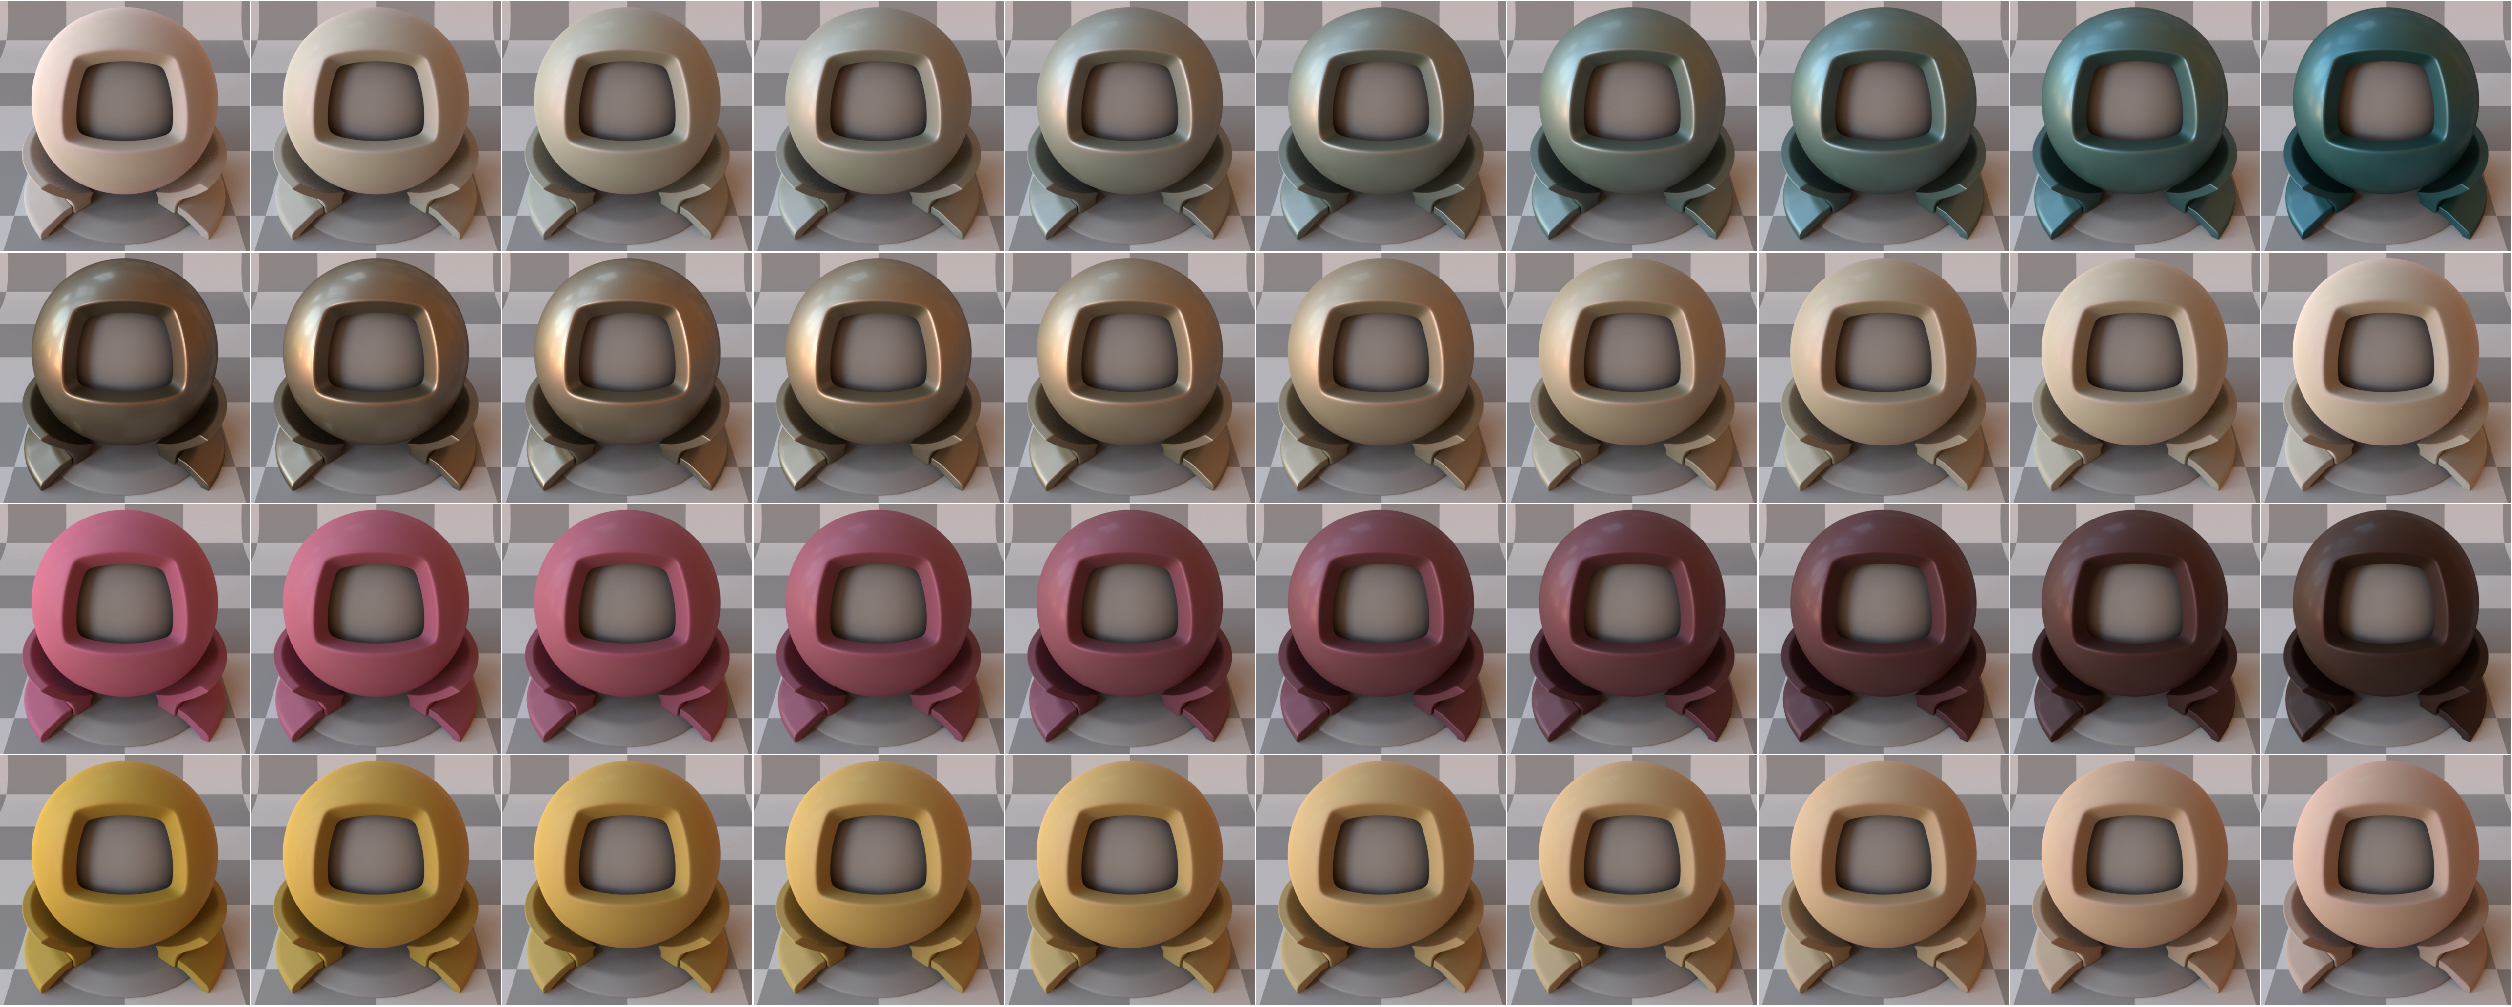
\includegraphics[width=0.9\linewidth]{Chapters/hyperbrdf-figs/interpolation_extended.pdf}

   \caption{BRDF editing through linear interpolation between the embeddings of two materials.}
   \label{fig:interpolation}
\end{figure*}


\subsection{Limitations and Future Work}\label{sec:limits}
\paragraph{Specular components:} Our network struggles with the estimation of specular components as shown in Figure~\ref{fig:imp_comp_upt} (last two rows). It is likely because of the high gap between the values of diffuse that are close to zero and the values of specular components that are arbitrarily high. We consider a separate estimation pipeline for each component within the network to improve the results.


\paragraph{BRDF editing:} Our BRDF editing approach is rather non-intuitive with an interpolation approach. Finding a map between the embeddings and certain attributes of the materials, such as diffuse/specular colors or haziness, can lead to more interactive BRDF editing. We plan to map our latent space to material parameter space so that users can easily edit materials through more interpretable parameters.

\paragraph{SVBRDF representations:} In this work, we focused on the task of generalizable neural representations for spatially uniform BRDFs. As the future work, we plan to extend our model to SVBRDF representations.
